\documentclass[11pt, a4Paper]{article}
\usepackage{graphicx}

\begin{document}

\title{Praktikumsbericht\\Schwingende Saite\\Versuch M13}
\author{Janosch Ehlers, Lenard Ansmann}
\date{20.12.2018}
\maketitle

\begin{center}
\textsc{Inhalt}
\end{center}

\begin{enumerate}
\item Ziel des Versuches
\item Theoretischer Hintergrund
\item Experimenteller Aufbau
\item Beobachtungen und Auswertung
\item Anhang
\end{enumerate}

\newpage
\section{Ziel des Versuches}
Hier wurde sich mit den Grundlagen der Wellenphysik beschäftigt. Unter anderem wurde das Konzept der stehenden Welle untersucht. Stehende Wellen spielen eine grundlegende Rolle in vielen Disziplinen der Physik. Unter anderem: in der Quantenmechanik, der Elektrodynamik und der Akustik. In unserem Versuch wurde eine Saite mithilfe der Lorentzkraft ausgelenkt und somit zum Schwingen gebracht. Unter Änderung der Spannkraft und der Stärke der Lorenzkraft wurde untersucht, welche Schwingung, welcher Harmonie in der Saite erzeugt wurde. 

\section{Theoretischer Hintergrund}
Wenn die Wellen Länge einer harmonischen Schwingung ein natürliches Vielfache einer Ausbreitungsrichtung ist, dann spricht man von einer stehenden Welle. Hier verändern alle Knotenpunkte diese Welle ihre Position nicht. Sie ,,Stehen'' förmlich. Bei stehenden Wellen kann allerdings in einer definierten Ausbreitungsrichtung nicht nur eine Frequenz eine stehende Welle gebildet werden. Diese bezeichnet man als die 2., 3., 4., 5., 6. ... Harmonische dieser Schwingung. Die 1. Harmonische einer Schwingung ist immer die Grundfrequenz. in diesem Fall hängt die Frequenz der stehenden Welle von der Wellenlänge, der Kraft auf die Saite, der Fläche des Querschnittes und der Dichte des Saite Materials ab. lso gilt: $$f=\frac{1}{\lambda}\sqrt{\frac{F}{\rho\cdot A}}$$ Da die Wellenlänge direkt mit der Länge der maximalen Ausbreitungsrichtung über $\lambda_n=\frac{n}{2L}$ zusammenhängt. Kann ein Zusammenhang zwischen der Frequenz und der Ordnungszahl der harmonischen Schwingung der stehenden Welle gebildet werden: $$f_n=\frac{n}{2L}\sqrt{\frac{F}{\rho\cdot A}}$$ In unserem Experiment wird die Saite über die Lorentzkraft in Schwingung versetzt. Dies ist eine Kraft die auf elektrische Ladungen Wirken, welche sich durch ein magnetisches Feld bewegen. Dabei gilt, $$F=IBs$$ wobei F die Kraft, I die Stromstärke und s die Polschubreite darstellt. Durch die Lorentzkraft wird hier Ladung in der Saite, und damit die Saite entsprechend der linken Hand Regel ausgelenkt. Diese sagt aus, dass die Stromflussrichtung, die Richtung der Magnetischfeldlinien und die Auslenkrichtung orthogonal zueinanderstehen.

\section{Experimenteller Aufbau}

Die Saite wurde durch einen Magneten hindurch zwischen einer Gitarrenmechanik (zum Spannen der Saite) und einem Kraftmessgerät gespannt. Die Saite war Teil eines Stromkreises, welcher einen Tonfrequenzgenerator als Stromquelle hat. Das Signal des Frequenzgenerators wurde daraufhin mit einem geeigneten Verstärker, verstärkt und über ein Ampermeter, einer Glühlampe und der Saite wieder zurück zur Signalquelle zurück geleitet. Ein Piezoelement, welches an der Saite angebracht wurde, misst die Auslenkung der Saite. Diese Schwingung wurde von einem Oszilloskop gemessen und sichtbar gemacht. Zum Vergleich wurde auch der Tonfrequenzgenerator mit dem Oszilloskop verbunden. Nun wurden in drei Versuchen das Schwingungsverhalten der Saite unter verändern der Rahmenbedingungen untersucht. In Versuch wurde bei einer Spannkraft von $10N$, und einer Stromstärke von $0,3A-0,5A$ die Harmonischen der Saite gesucht. In einem zweiten Experiment sollte die Abhängigkeit der Grundfrequenz der Saite von der Spannkraft untersucht werden. Hier wurde die Spannkraft in einem Bereich von $2N-24N$ variiert und die harmonische Schwingung mittels Einstellen der Erregerfrequenz gesucht. Die Stromstärke blieb unverändert. In einem dritten Versuch sollte nun bei einer Erregerfrequenz von $1kHz$, einer Spannkraft von $8N-10N$ und einer Stromstärke von $0,3A-1A$ mittels Verschieben des Magneten die harmonische Ordnungszahl bestimmt werden.  

\newpage
\section{Beobachtungen und Auswertung}

Die Saite wurde im ersten Versuch bei einer Spannkraft von 10 N und von 270 mA Strom durchflossen. Hier konnten folgende Werte beobachtet werden:\\
\begin{enumerate}
\item Harmonische $(49,5\ \pm 0,1) Hz$
\item Harmonische $(96,1\ \pm 0,1) Hz$
\item Harmonische $(150,2\ \pm 0,1) Hz$
\item Harmonische $(198,0\ \pm 0,1) Hz$
\item Harmonische $(0,20\ \pm 0,01) KHz$ 
\item Harmonische $(0,24\ \pm 0,01) KHz$
\end{enumerate}
Der Sprung in den Einheiten ist der Anzeige des Tonfrequenzgenerators geschuldet. Dieser war leider nur in der Lage die Frequenz bis 200 Hz in 0,1 Hz Schritten anzuzeigen. Das nächsthöhere Level die Frequenz anzuzeigen hatte den Nachteil, dass die Auflösung hier nur 0,01 Khz betrug. Wollen wir nun die gemessenen Werte mit den Theoretischen vergleichen, nutzen wir einfach die Oben genannte Formel: $$f_n\ =\ \frac{n}{2L}\cdot\sqrt{\frac{F}{\rho\cdot A}}$$ Nun setzen wir die gegebenen Werte ein:\\ L=0,9m F=10N $\rho$=8,59$\frac{g}{cm^3}$ A=$\pi\cdot (\frac{53\cdot 10^{-6}}{2 })^2$ $$f_n\ =\ \frac{2\cdot 0,9m}{n}\cdot\sqrt{\frac{10N}{8,59\frac{g}{cm^3}\cdot \pi\cdot (\frac{53\cdot 10^{-6}}{2 })^2}}$$ wir erhalten eine Gleichung, in der wir in Abhängigkeit der harmonischen Ordnungszahl die Frequenz errechnen können. Der Fehler der jeweiligen Werte ist wie folgt definiert: $$\Delta f\ =\ \sum \limits_{K=1}^{N} \left| \frac{\delta f}{\delta x}\cdot \Delta x \right|$$ Die Messfehler der eigenen Instrumente sind Folgende: $\Delta N = \pm 0,5N$; $\Delta L = \pm 0,5 mm $; $\Delta d = \pm 10^{-6}m$
Fangen wir an die Partiellen Ableitungen zu bilden: 
$$\frac{\delta f}{\delta L}=\left[\frac{n}{2L}\sqrt{\frac{4F}{\rho\pi d^2}} \right]'=\left[L^{-1}\cdot \frac{n}{2}\sqrt{\frac{4F}{\rho\pi d^2}} \right]'=-L^{-2}\frac{n}{2}\sqrt{\frac{4F}{\rho\pi d^2}} = \frac{-n}{2L^2}\sqrt{\frac{4F}{\rho\pi d^2}}$$ 
$$\frac{\delta f}{\delta F}=\left[\frac{n}{2L}\sqrt{\frac{4F}{\rho\pi d^2}} \right]'=\left[\frac{n}{2L}\cdot(\frac{4F}{\rho\pi d^2})^{\frac{1}{2}} \right]' =\left[\frac{n}{2L}\cdot(\frac{4}{\rho\pi d^2})^{\frac{1}{2}}\cdot F^{\frac{1}{2}} \right]'$$ $$ =\frac{n}{2L}\cdot(\frac{4}{\rho\pi d^2})^{\frac{1}{2}}\cdot \frac{F^{-\frac{1}{2}}}{2} =\frac{n}{4LF^{\frac{1}{2}}}\cdot(\frac{4}{\rho\pi d^2})^{\frac{1}{2}}$$
$$\frac{\delta f}{\delta d}=\left[\frac{n}{2L}\sqrt{\frac{4F}{\rho\pi d^2}} \right]' =\left[\frac{n}{2L}\cdot (\frac{4F}{\rho\pi d^2})^{\frac{1}{2}} \right]' =\left[\frac{n}{2L}\cdot (\frac{4F}{\rho\pi})^{\frac{1}{2}}\cdot (\frac{1}{d^2})^{\frac{1}{2}} \right]' =\left[\frac{n}{2L}\cdot (\frac{4F}{\rho\pi})^{\frac{1}{2}}\cdot d^{-1} \right]'$$ $$ =\frac{n}{2L}\cdot (\frac{4F}{\rho\pi})^{\frac{1}{2}}\cdot (-d^{-2}) =\frac{n}{-2d^2L}\cdot (\frac{4F}{\rho\pi})^{\frac{1}{2}}$$
Diese Terme können nun in die oben genannte Formel eingesetzt werden: $$\Delta f=\left|\frac{-n}{2L^2}\sqrt{\frac{4F}{\rho\pi d^2}}\cdot\Delta L\right|+\left|\frac{n}{4LF^{\frac{1}{2}}}\cdot(\frac{4}{\rho\pi d^2})^{\frac{1}{2}}\cdot \Delta F\right|+\left|\frac{n}{-2d^2L}\cdot (\frac{4F}{\rho\pi})^{\frac{1}{2}}\cdot\Delta d\right|$$

Die Theoretischen Werte können der folgenden Tabelle, aber auch der Abbildung 2, entnommen werden:
\begin{flushleft}
\textsc{Tabelle 1: Theoretische Werte Versuch 1}
\end{flushleft}

\begin{tabular}{cc}
Schwingung & Frequenz $\pm$ Fehler\\
\hline
1. Harmonische & $(40,5692726752962 \pm 18,2476676152721)$Hz\\
2. Harmonische & $(81,1385453505924 \pm 36,4953352305443)$Hz\\
3. Harmonische & $(121,707818025889 \pm 39,4338433457046)$Hz\\
4. Harmonische & $(162,277090701185 \pm 72,9906704610885)$Hz\\
5. Harmonische & $(202,846363376481 \pm 91,2383380763606)$Hz\\
6. Harmonische & $(243,415636051777 \pm 109,486005691633)$Hz\\
\end{tabular}\\

Die Messergebnisse liegen alle innerhalb der Fehlerbereiche der theoretischen Ergebnisse. Allerdings muss erwähnt werden, dass mit Steigender harmonischer Ordnungszahl sich zum einen der theoretische Mittelwert unseren Messergebnissen immer weiter annähert, sich allerdings auch der errechnete Fehlerbereich auf die Zweifache Größe des intuitiv erwarteten Intervalls ansteigt. So kann gesagt werden, dass es bei steigender harmonischer Ordnungszahl der Vergleich mit dem hier errechneten theoretischen Wert nicht mehr so aussagekräftig ist.\\Die Lorentzkraft, bei diesem Versuch, errechnet sich aus: $$F=IBs=0,47A\cdot 0,017m\cdot 0,25T=1,41\cdot 10^{-3}N$$ Die Ergebnisse des Versuchs 2 sind in Abbildung 3, aber auch in Tabelle 2 dargestellt, da die diskreten Messdaten hier viel anschaulicher sind.\\
\begin{flushleft}
\textsc{Tabelle 2: Messung und Grundfrequenz von Versuch 2 bei 0,751A}
\end{flushleft}
\begin{tabular}{c|cc|cc}
 & Aufwärts & & Abwärts & \\
Kraft (N) & Frequenz (kHz) & Grundfrequenz & Frequenz (kHz) & Grundfrequenz\\
\hline
$25$ & $0,306$ & $0,102$ & $0,307$ & $0,102\overline{3}$\\
$23$ & $0,293$ & $0,097\overline{6}$ & $0,294$ & $0,098$\\
$21$ & $0,281$ & $0,093\overline{6}$ & $0,281$ & $0,093\overline{6}$\\
$19$ & $0,267$ & $0,089$ & $0,268$ & $0,089\overline{3}$\\
$17$ & $0,253$ & $0,084\overline{3}$ & $0,254$ & $0,084\overline{6}$\\
$15$ & $0,24$ & $0,08$ & $0,239$ & $0,079\overline{6}$\\
$13$ & $0,223$ & $0,074\overline{3}$ & $0,223$ & $0,074\overline{3}$\\
$11$ & $0,206$ & $0,068\overline{6}$ & $0,204$ & $0,068$\\
$9$ & $0,183$ & $0,061$ & $0,184$ & $0,061\overline{3}$\\
$7$ & $0,162$ & $0,054$ & $0,163$ & $0,054\overline{3}$\\
$5$ & $0,136$ & $0,045\overline{3}$ & $0,138$ & $0,046$\\
$3$ & $0,117$ & $0,039$ & $0,115$ & $0,038\overline{3}$\\
$2$ & $0,098$ & $0,032\overline{6}$ & $0,118$ & $0,039$\\
\end{tabular}\\
Die Änderungsrate der Grundfrequenz bei der Aufwärtsbewegung ist $(0,005\overline{7} \pm 0,002\overline{8})kHz$, während bei der Abwärtsbewegung eine Änderungsrate von $(0,00525
\pm 0,00308\overline{3})kHz$ zu errechnen ist. Es ist deutlich zu erkennen, dass Die Aufwärtsmessung hier geringfügig genauer war. Die Abweichung beider Messreihen bei gleicher Spannkraft beträgt $(0,00036\overline{1} \pm 0,00036\overline{1})kHz$ Die Unterschiede in den Messungen können sowohl dem menschlichen Fehler als auch dem Aufbau zugeordnet werden. Sowohl das Erkennen der harmonischen Frequenz ist nur mit einer bestimmten Ungenauigkeit möglich und auch die Tatsache das die Gitarrensaite nicht gleichmäßig spannbar ist verursacht einige Fehler. Des Weiteren hat das Kraftmessgerät einen vergleichsweise hohen Fehler, somit kann leicht beim zweiten Durchlauf eine andere Kraft eingestellt werden.\\
Im dritten Experiment versuchten wir die Harmonische Ordnungszahl einer gegebenen Schwingung zu bestimmen. Hier wurde eine Spannkraft von $9 N$, eine Stromstärke von $0,69A$ und eine Frequenz von $1,002 kHz$ eingestellt. Gemessen von der Gitarrenspannvorrichtung aus wurden an folgenden Punkten Knotenpunkte gemessen: $4cm, 8cm, 13cm, 16,5cm, 20,5cm, 25cm, 29cm,$\\$ 33,5cm, 38cm, 42cm, 46cm, 51cm, 55cm, 59,5cm, 63,5cm, 68cm, 72,5cm,$\\$ 76,5cm, 80,5cm, 85cm$ sowohl an Punkt $0cm$ als auch an Punkt $90cm$ ist ein Knotenpunkt, der nicht auf diese Art und Weise messbar ist. Es sind also 22 Knotenpunkte. Da die harmonische Ordnungszahl (n) über die Knotenpunkte (kn) mit $n+1=kn$ definiert ist, errechnet sich für $n=kn-1=22-1=21$ die 21. Harmonische oder die 20. Oberschwingung. 
 
\section{Anhang}
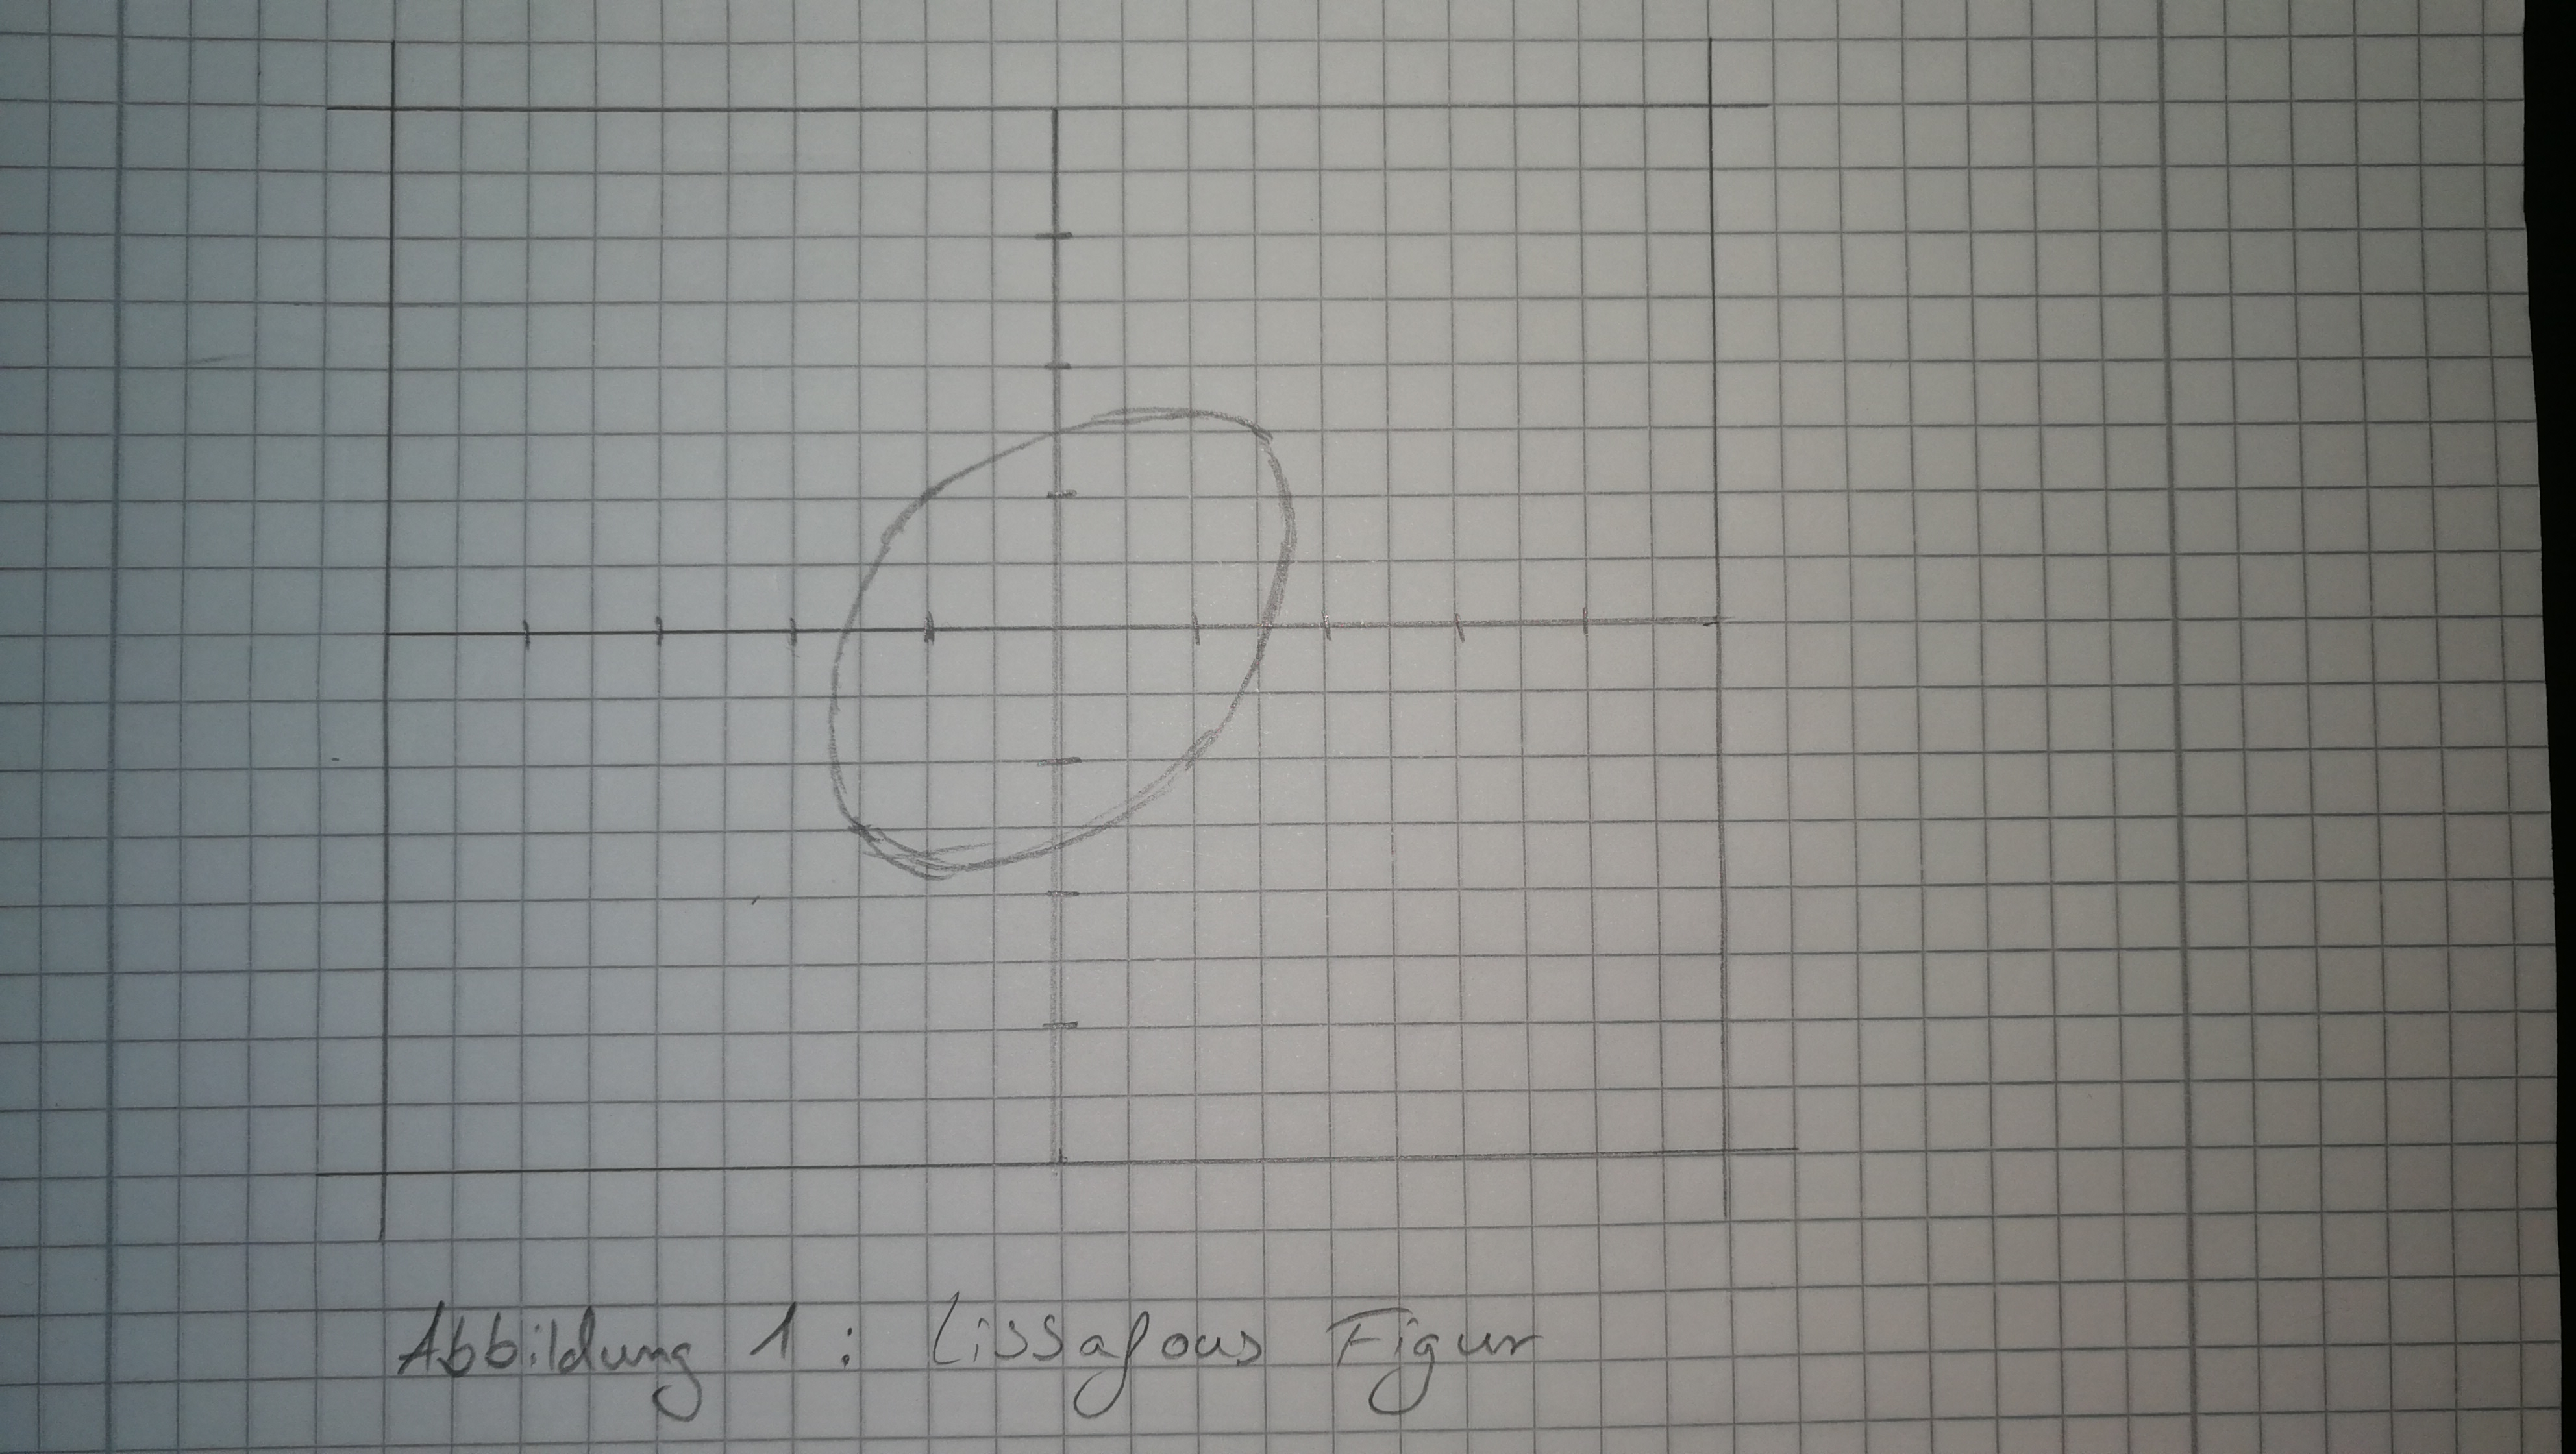
\includegraphics[scale=0.1]{Abb1.jpg}\\
Abb.1 \\
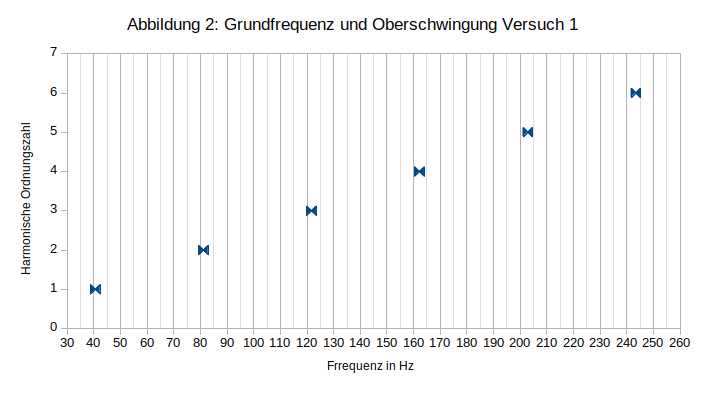
\includegraphics[scale=0.7]{Abb2.png}\\
Abb.2 \\
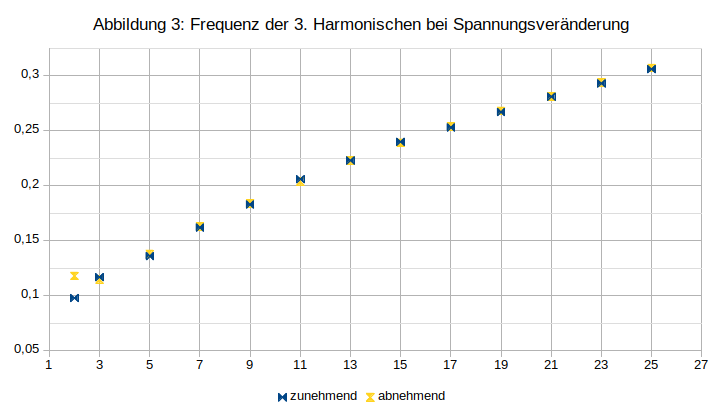
\includegraphics[scale=0.7]{Abb3.png}\\
Abb.3 \\
\end{document}